\documentclass[a4paper,12pt]{article}

\usepackage[T2A]{fontenc}
\usepackage[utf8]{inputenc}
\usepackage[russian]{babel}

\usepackage{amsmath}
\usepackage{amssymb}
\usepackage{amsfonts}

\usepackage[margin=2.5cm]{geometry}
\usepackage{graphicx}
\usepackage[usenames,dvipsnames,svgnames,table]{xcolor}

\usepackage{hyperref}
\hypersetup{
    colorlinks=true,
    linkcolor=blue,
    filecolor=magenta,      
    urlcolor=cyan,
    pdftitle={Лабораторная работа по ТФКП},
    pdfpagemode=FullScreen,
}

\usepackage{listings}
\lstdefinestyle{mypython}{
    language=Python,
    basicstyle=\ttfamily\scriptsize,
    keywordstyle=\color{blue}\bfseries,
    stringstyle=\color{red},
    commentstyle=\color{green!60!black},
    numbers=left,
    numberstyle=\tiny\color{gray},
    stepnumber=1,
    numbersep=8pt,
    showspaces=false,
    showstringspaces=false,
    tabsize=4,
    frame=single,
    rulecolor=\color{black},
    breaklines=true,
    breakatwhitespace=false,
    captionpos=b,
    xleftmargin=15pt,
    xrightmargin=5pt,
    framexleftmargin=12pt,
    backgroundcolor=\color{gray!5},
    literate=%
        {а}{{\cyra}}1 {б}{{\cyrb}}1 {в}{{\cyrv}}1 {г}{{\cyrg}}1 {д}{{\cyrd}}1
        {е}{{\cyre}}1 {ё}{{\cyrie}}1 {ж}{{\cyrzh}}1 {з}{{\cyrz}}1 {и}{{\cyri}}1
        {й}{{\cyrishrt}}1 {к}{{\cyrk}}1 {л}{{\cyrl}}1 {м}{{\cyrm}}1 {н}{{\cyrn}}1
        {о}{{\cyro}}1 {п}{{\cyrp}}1 {р}{{\cyrr}}1 {с}{{\cyrs}}1 {т}{{\cyrt}}1
        {у}{{\cyru}}1 {ф}{{\cyrf}}1 {х}{{\cyrh}}1 {ц}{{\cyrc}}1 {ч}{{\cyrch}}1
        {ш}{{\cyrsh}}1 {щ}{{\cyrshch}}1 {ъ}{{\cyrhrdsn}}1 {ы}{{\cyrery}}1
        {ь}{{\cyrsftsn}}1 {э}{{\cyrerev}}1 {ю}{{\cyryu}}1 {я}{{\cyrya}}1
        {А}{{\CYRA}}1 {Б}{{\CYRB}}1 {В}{{\CYRV}}1 {Г}{{\CYRG}}1 {Д}{{\CYRD}}1
        {Е}{{\CYRE}}1 {Ё}{{\CYRIE}}1 {Ж}{{\CYRZH}}1 {З}{{\CYRZ}}1 {И}{{\CYRI}}1
        {Й}{{\CYRISHRT}}1 {К}{{\CYRK}}1 {Л}{{\CYRL}}1 {М}{{\CYRM}}1 {Н}{{\CYRN}}1
        {О}{{\CYRO}}1 {П}{{\CYRP}}1 {Р}{{\CYRR}}1 {С}{{\CYRS}}1 {Т}{{\CYRT}}1
        {У}{{\CYRU}}1 {Ф}{{\CYRF}}1 {Х}{{\CYRH}}1 {Ц}{{\CYRC}}1 {Ч}{{\CYRCH}}1
        {Ш}{{\CYRSH}}1 {Щ}{{\CYRSHCH}}1 {Ъ}{{\CYRHRDSN}}1 {Ы}{{\CYRERY}}1
        {Ь}{{\CYRSFTSN}}1 {Э}{{\CYREREV}}1 {Ю}{{\CYRYU}}1 {Я}{{\CYRYA}}1
}
\lstset{style=mypython}

\usepackage{titlesec}
\titleformat{\section}
  {\normalfont\Large\bfseries}{\thesection}{1em}{}
\titleformat{\subsection}
  {\normalfont\large\bfseries}{\thesubsection}{1em}{}

\begin{document}

\begin{titlepage}
    \centering
    \normalsize
    Федеральное государственное автономное образовательное учреждение \\
    высшего образования «Национальный исследовательский университет \\
    ИТМО» \\[0.8cm]
    Факультет программной инженерии и компьютерной техники \\[2.5cm]
    
    \LARGE
    Лабораторная работа \\
    \normalsize
    по ТФКП \\[1.2cm]
    
    \Large
    \textbf{Построение и визуализация \\ фрактальных множеств}
    
    \vfill
    
    \hfill
    \begin{tabular}{l}
        Выполнили: \\
        студенты потока 22.4 \\[0.3cm]
        \textit{Шумахер Демид Сергеевич} \\
        \textit{Михайлов Петр Сергеевич} \\
        \textit{Соболев Егор Викторович} \\
    \end{tabular}
    \hspace{1cm}
    
    \vfill
    
    \centering
    Санкт-Петербург - 2025
\end{titlepage}

\pagestyle{plain}
\setcounter{page}{2}

\section*{\textbf{Оглавление}}
\addcontentsline{toc}{section}{Оглавление}

{\bfseries
\noindent 1 \quad Задание \hfill \hyperlink{sec:1}{3} \\
\noindent 2 \quad Доказательство первого свойства множества Мандельброта \hfill \hyperlink{sec:2}{4} \\
\noindent 3 \quad Доказательство второго свойства множества Мандельброта \hfill \hyperlink{sec:3}{5} \\
\noindent 4 \quad Код функции для построения множеств Мандельброта \hfill \hyperlink{sec:4}{7} \\
\noindent 5 \quad Изображения множества Мандельброта с разными параметрами \hfill \hyperlink{sec:5}{8} \\
\noindent 6 \quad Код функции для построения множеств Жюлиа \hfill \hyperlink{sec:6}{10} \\
\noindent 7 \quad Изображения множества Жюлиа с разными параметрами \hfill \hyperlink{sec:7}{11} \\
\noindent 8 \quad Фрактал «Горящий корабль» \hfill \hyperlink{sec:8}{13} \\
}

\clearpage

\hypertarget{sec:1}{}
\section{\textbf{Задание}}
\begin{enumerate}
    \item Докажите свойства 1 и 2 для множества Мандельброта.
    \item Напишите программу, которая будет строить визуализацию множества Мандельброта. Выберите разумные ограничения, поварьируйте максимальное количество итераций. Попробуйте приблизить отдельные части множества, чтобы увидеть фрактальную структуру.
    \item Напишите программу, которая по заданному $c$ строит заполненное множество Жюлиа. Поварьируйте максимальное количество итераций, попробуйте пронаблюдать фрактальную структуру, рассмотрите множество при разных $c$. (Например, красиво получается при $c=0.5251993+i\cdot0.5251993)$.
    \item Найдите какой-нибудь неразобранный фрактал (например, бассейны Ньютона). Опишите его структуру, построение. Нарисуйте визуализации. Будьте готовы выступить с докладом перед своими одногруппниками.
\end{enumerate}

\clearpage

\hypertarget{sec:2}{}
\section{\textbf{Доказательство первого свойства множества Мандельброта}}

\begin{enumerate}
    \item $M=\{c\in\mathbb{C} \mid \exists M\in\mathbb{R} : \forall n\in\mathbb{N} \ |z_{n+1}=z_{n}^{2}+c| \le M\}$ — множество Мандельброта, где $z_{n}$ — последовательность комплексных чисел, $z_{0}=0$, а $M$ — конечное вещественное число.
    \item $\overline{c}$ — комплексно сопряжённое к $c$, $z'_{n}$ — последовательность, построенная для $\overline{c}$.
    \item Требуется доказать, что если $c\in Q$, то $\overline{c}\in Q$.
    \item По определению множества, $\overline{c}\in Q \Leftrightarrow |z'_{n+1}=z'^{2}_{n}+\overline{c}|<M$.
    \item Докажем, что $z'_{n}=\overline{z_{n}}$ по индукции:
    
    \textbf{База:} $z_{0}=z'_{0}=0$. 
    
    \textbf{Переход:} Пусть $z_{n}=x+iy$, $c=a+ib$. Тогда
    \begin{align*}
        z'_{n+1} &= z'^{2}_{n}+\overline{c} = (x-iy)^{2}+(a-ib) \\
        &= x^{2}-y^{2}-i2xy+a-ib \\
        &= (x^{2}-y^{2}+a)-i(2xy+b) \\
        &= \overline{((x^{2}-y^{2}+a)+i(2xy+b))} = \overline{(z_{n}^{2}+c)} = \overline{z_{n+1}}.
    \end{align*}
    
    \textbf{Вывод:} $z'_{n}=\overline{z_{n}} \Rightarrow |z'_{n}|=|z_{n}|$. Следовательно, если $c\in Q$, то $|z_{n}|<M$, и, значит, $|\overline{z_{n}}|<M$, то есть $\overline{c}\in Q$.
\end{enumerate}

\clearpage

\hypertarget{sec:3}{}
\section{\textbf{Доказательство второго свойства множества Мандельброта}}

\textbf{Определение:} Точка $c$ принадлежит множеству Мандельброта тогда и только тогда, когда рекуррентная последовательность
$$
z_{n+1}=z_{n}^{2}+c, \quad z_{0}=0
$$
остаётся ограниченной, то есть существует $M>0$, такое что $\forall n \in \mathbb{N}$ выполняется $|z_{n}|<M$.

\textbf{Цель:} Доказать, что если $|c|>2$, то последовательность $z_{n}$ не ограничена, а значит, $c$ не принадлежит множеству.

\textbf{Шаг 1.} Докажем, что последовательность $|z_{n}|$ начиная с $n=1$ строго возрастает и все её члены больше 2.

\textbf{База индукции $(n=1)$:} $z_{0}=0$, $z_{1}=z_{0}^{2}+c=c$, значит $|z_{1}|=|c|>2$. Далее
$$
z_{2}=z_{1}^{2}+c=c^{2}+c,
$$
и по неравенству треугольника:
$$
|z_{2}|=|c^{2}+c|\ge |c^{2}|-|c|=|c|^{2}-|c|=|c|(|c|-1).
$$
Так как $|c|>2$, имеем $|c|-1>1$, следовательно $|z_{2}|>|c|=|z_{1}|>2$.

\textbf{Индукционное предположение:} Для некоторого $n\ge 2$ верно $|z_{n}|>|z_{n-1}|>2$.

\textbf{Индукционный переход $(n\to n+1)$:}
$$
|z_{n+1}|=|z_{n}^{2}+c|\ge |z_{n}|^{2}-|c|=|z_{n}|\left(|z_{n}|-\frac{|c|}{|z_{n}|}\right).
$$
Так как $|z_{n}|>|c|>2$, то $\frac{|c|}{|z_{n}|}<1$ и $(|z_{n}|-\frac{|c|}{|z_{n}|})>1$, откуда $|z_{n+1}|>|z_{n}|>2$.

\textbf{Вывод Шага 1:} Последовательность $|z_{n}|$ начиная с $n=1$ строго возрастает, и все её члены больше 2.

\textbf{Шаг 2.} Покажем, что последовательность $|z_{n}|$ не может быть ограниченной.

Предположим противное: $|z_{n}|$ ограничена сверху. Тогда, по теореме Вейерштрасса, существует предел $M=\lim_{n\to\infty}|z_{n}|<\infty$.

Из неравенства треугольника имеем
$$
|z_{n+1}|\ge |z_{n}|^{2}-|c|,
$$
следовательно
$$
|z_{n+1}|-|z_{n}|\ge |z_{n}|^{2}-|z_{n}|-|c|=:f(|z_{n}|).
$$
Так как $|z_{n}|\ge |c|>2$, то $f(|z_{n}|)\ge f(|c|)=|c|^{2}-2|c|>0$. Обозначим $\delta = |c|^{2}-2|c|$.

Таким образом, для всех $n\ge 1$ выполняется
$$
|z_{n+1}| \ge |z_{n}|+\delta.
$$

Теперь, если $\lim_{n\to\infty}|z_{n}|=M$, то по определению предела существует $N$, такое что $\forall n\ge N$:
$$
M-\varepsilon<|z_{n}|<M+\varepsilon.
$$
Выберем $\varepsilon$ так, чтобы $0<\varepsilon<\frac{\delta}{2}=\frac{|c|^{2}-2|c|}{2}$.

Тогда для такого $n$:
$$
|z_{n+1}| \ge |z_{n}|+\delta > (M-\varepsilon)+\delta = M + (\delta-\varepsilon).
$$
Так как $\delta-\varepsilon>\varepsilon$, получаем $|z_{n+1}|>M+\varepsilon$, что противоречит ограниченности последовательности.

\textbf{Вывод Шага 2:} Предположение о существовании конечного предела $M$ приводит к противоречию. Следовательно, последовательность $|z_{n}|$ неограничена.

\textbf{Заключение:} Если $|c|>2$, то последовательность $z_{n}$ не ограничена, следовательно, точка $c$ не принадлежит множеству Мандельброта. \qed

\clearpage

\hypertarget{sec:4}{}
\section{\textbf{Код функции для построения множеств Мандельброта}}

\begin{lstlisting}[caption={Функция для построения множества Мандельброта}, label={lst:mandelbrot}]
def mandelbort_matrix(fractal_params, iterations, borders, density):
    z0 = fractal_params.get("z0") 
    r = fractal_params.get("r")
    
    plane_start, plane_end = borders
    
    # Вектор действительных частей комплексной плоскости
    re_vec = np.linspace(plane_start.real, plane_end.real, density,
                         dtype=np.float32)
    
    # Вектор мнимых частей комплексной плоскости
    im_vec = np.linspace(plane_start.imag, plane_end.imag, density,
                         dtype=np.float32) * 1j
                         
    # Формируем дискретную комплексную плоскость точек С
    # с помощью декартового сложения двух векторов
    # В итоговой плоскости получаем density^2 точек
    plane = np.add.outer(im_vec, re_vec)
    
    # Результирующая матрица для вывода и окраски
    output = np.zeros(plane.shape, dtype='uint16')
    
    # Промежуточная матрица из комплексных чисел для формирования
    # последовательности, заполненная z0
    # В ней будем хранить n-ые члены последовательности для всех
    # подходящий точек c (plane)
    z = np.full(plane.shape, z0, np.complex64) 
    
    for i in range(iterations):
        # Матрица из точек, в которых текущее z еще не "убежало"
        mask = np.less(np.abs(z), r)
        # Чем больше чисел попало в точку, тем большее число для
        # данной точке будет в результирующей матрице
        output[mask] = i
        
        # Формируем следующий член последовательности для чисел,
        # которые отвечают радиусу
        # z_{n+1} = z_n^2 + c
        z[mask] = z[mask]**2 + plane[mask]
        
    return output
\end{lstlisting}
Полный код вы можете увидеть на \href{https://github.com/Axe-On-You/tfkp-lab1}{Github}.

\clearpage

\hypertarget{sec:5}{}
\section{\textbf{Изображения множества Мандельброта с разными параметрами}}

\begin{figure}[h!]
    \centering
    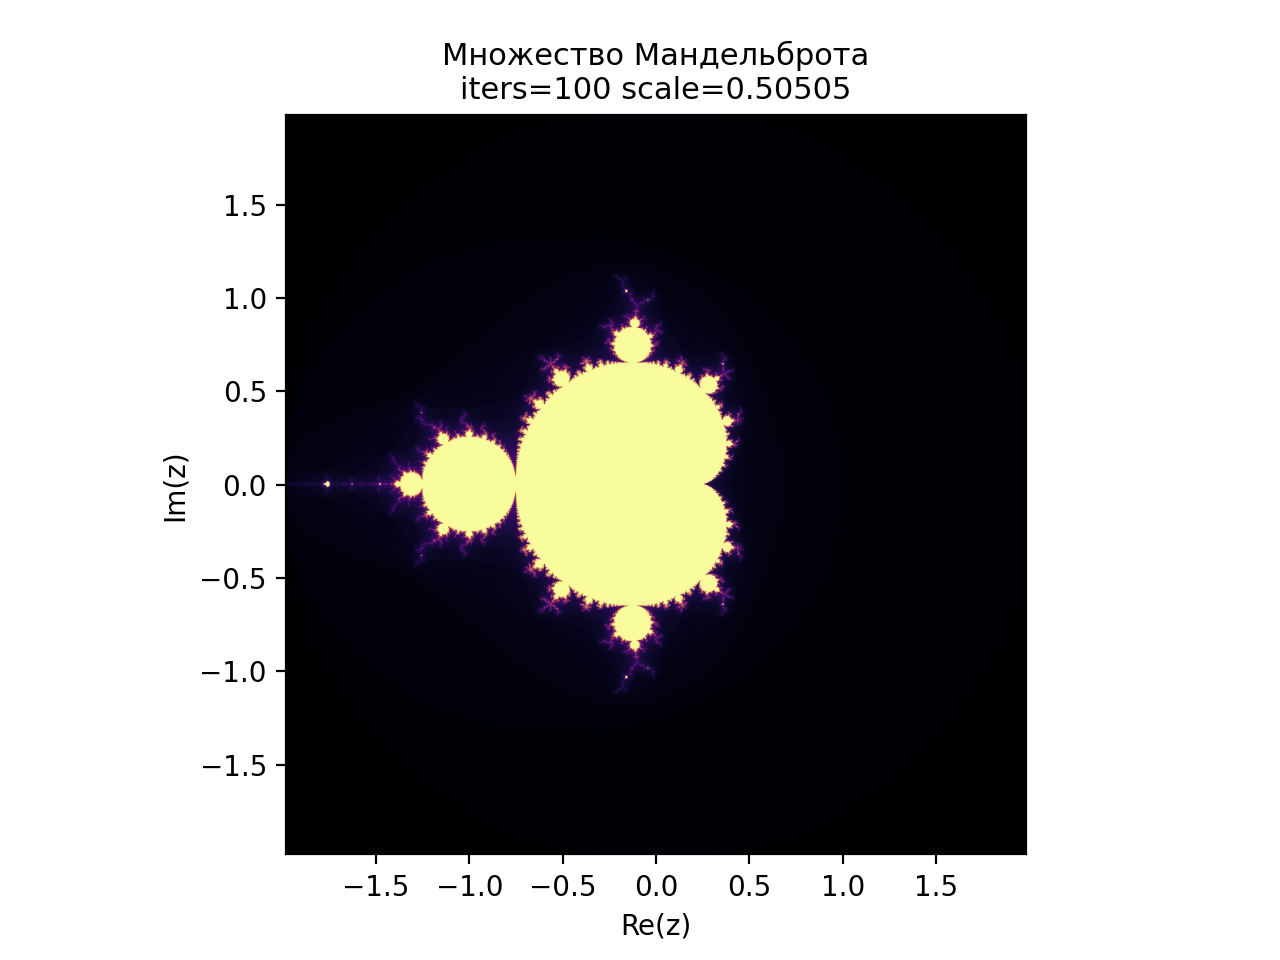
\includegraphics[width=0.9\textwidth]{mandelbrot_main.png}
    
    \vspace{0.5cm}
    
    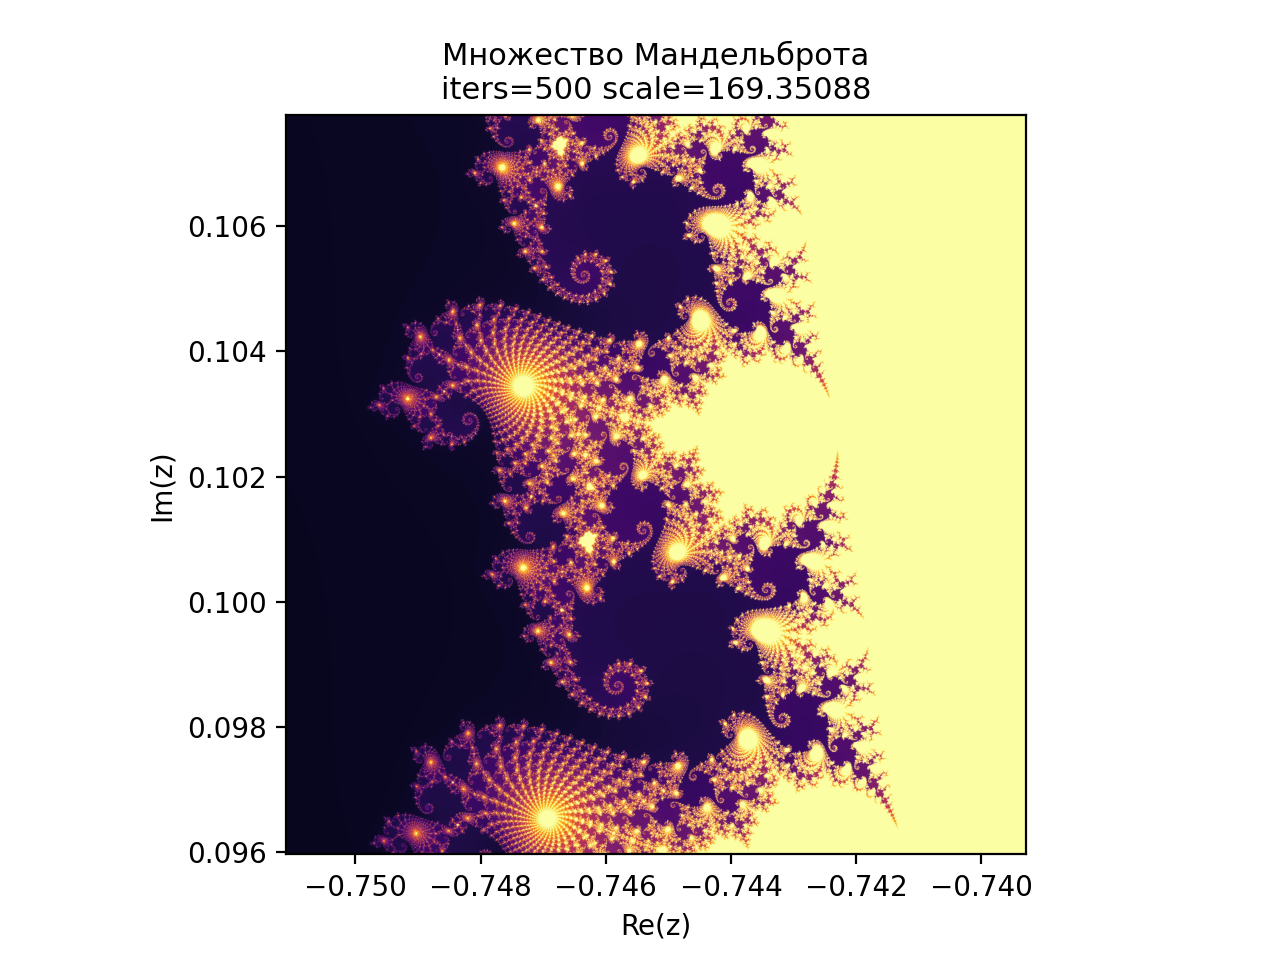
\includegraphics[width=0.9\textwidth]{mandelbrot_seahorse.png}
\end{figure}

\clearpage

\begin{figure}[h!]
    \centering
    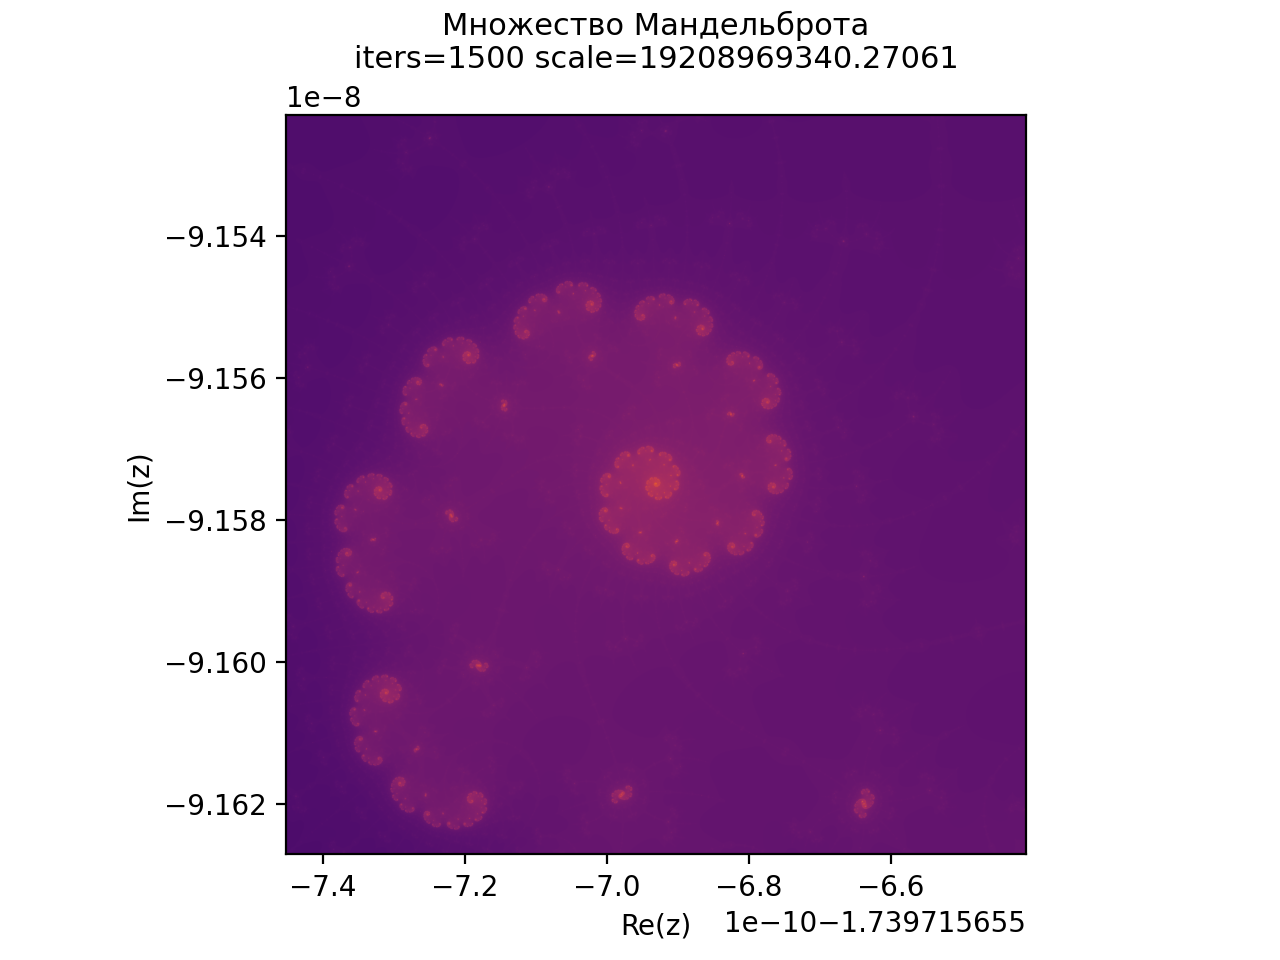
\includegraphics[width=1\textwidth]{mandelbrot_wormhole.png}
    
    \vspace{0.5cm}
    
    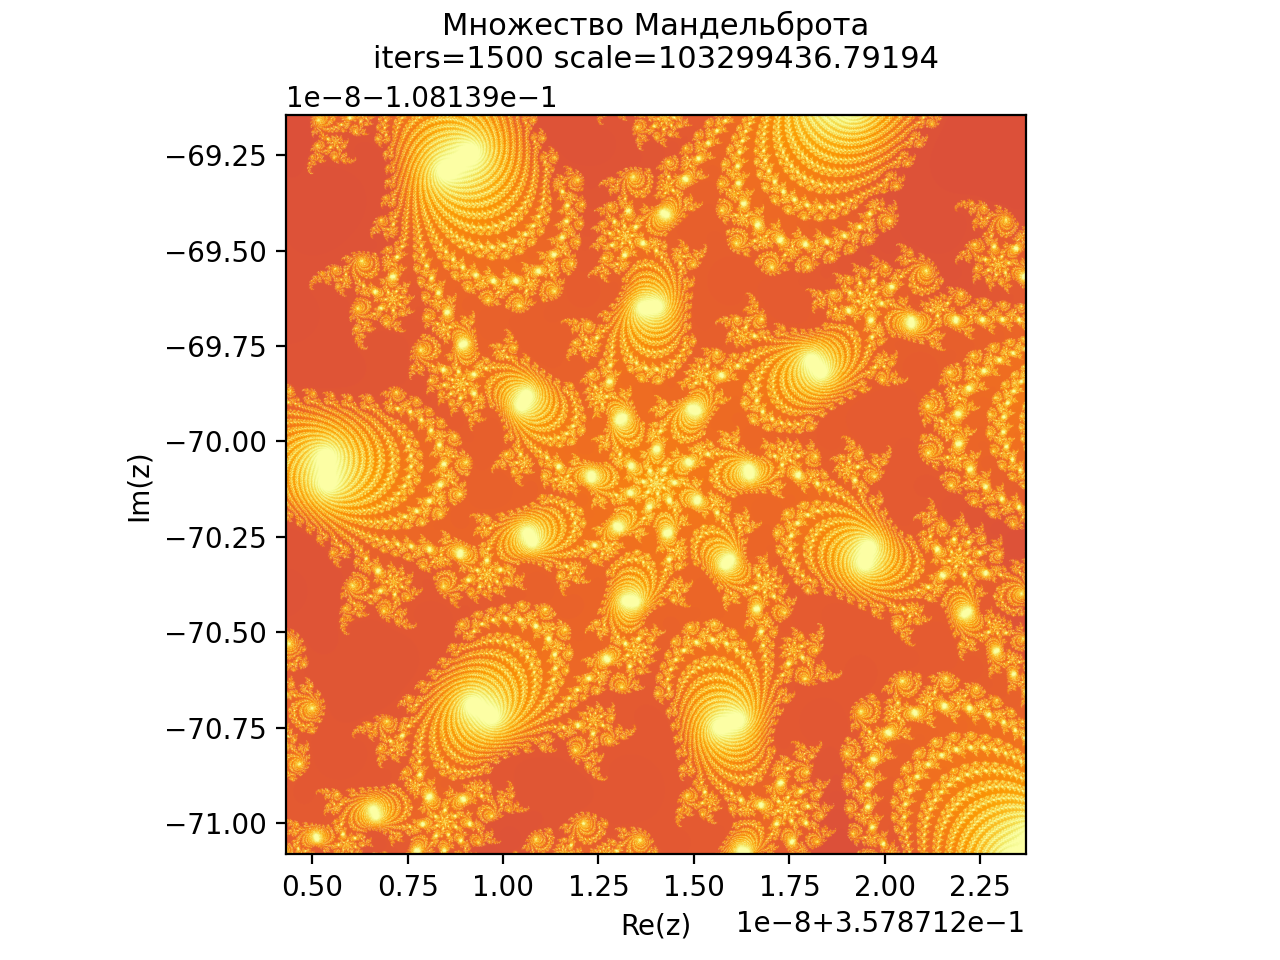
\includegraphics[width=1\textwidth]{mandelbrot_carousel.png}
\end{figure}

\clearpage

\hypertarget{sec:6}{}
\section{\textbf{Код функции для построения множеств Жюлиа}}

\begin{lstlisting}[caption={Функция для построения множества Жюлиа}, label={lst:julia}]
def julia_matrix(fractal_params, iterations, borders, density):
    c = fractal_params.get("c")
    r = fractal_params.get("r")
    plane_start, plane_end = borders

    # Выбор оптимального r
    # Имеем: r^2 - r >= |c|
    # r >= (1 +- sqrt(1 + 4|c|))/2 + eps
    # Если передано значение r меньшее, чем оптимальное - оставляем как есть для исследования области с меньшим r
    # Иначе рассчитываем оптимальное значение, так как исследование области с большим r не имеет смысла
    r = min(r, (1 + np.sqrt(1+4*np.abs(c)))/2 + 0.01)

    # Вектор действительных частей комплексной плоскости
    re_vec = np.linspace(plane_start.real, plane_end.real, density, dtype=np.float64)
    # Вектор мнимых частей комплексной плоскости
    im_vec = np.linspace(plane_start.imag, plane_end.imag, density, dtype=np.float64) * 1j
    # Формируем дискретную комплексную плоскость с помощью декартового сложения двух векторов
    # В итоговой плоскости получаем density^2 точек
    z = np.add.outer(im_vec, re_vec)

    # Результирующая матрица для вывода и окраски
    output = np.zeros(z.shape, dtype='uint16')

    for i in range(iterations):
        # Матрица из точек, в которых текущее z еще не "убежало"
        mask = np.less(np.abs(z), r)
        # Чем больше чисел попало в точку, тем большее число для данной точке будет в результирующей матрице
        output[mask] = i
        # Формируем следующий член последовательности для чисел, которые отвечают радиусу
        # z_{n+1} = z_n ^ 2 + c (const)
        # Аналогично первому фракталу, но используем c как const и применяем функцию к каждой точке z
        z[mask] = z[mask] ** 2 + c
    return output
\end{lstlisting}
Полный код вы можете увидеть на \href{https://github.com/Axe-On-You/tfkp-lab1}{Github}.

\clearpage

\hypertarget{sec:7}{}
\section{\textbf{Изображения множества Жюлиа с разными параметрами}}

\begin{figure}[h!]
    \centering
    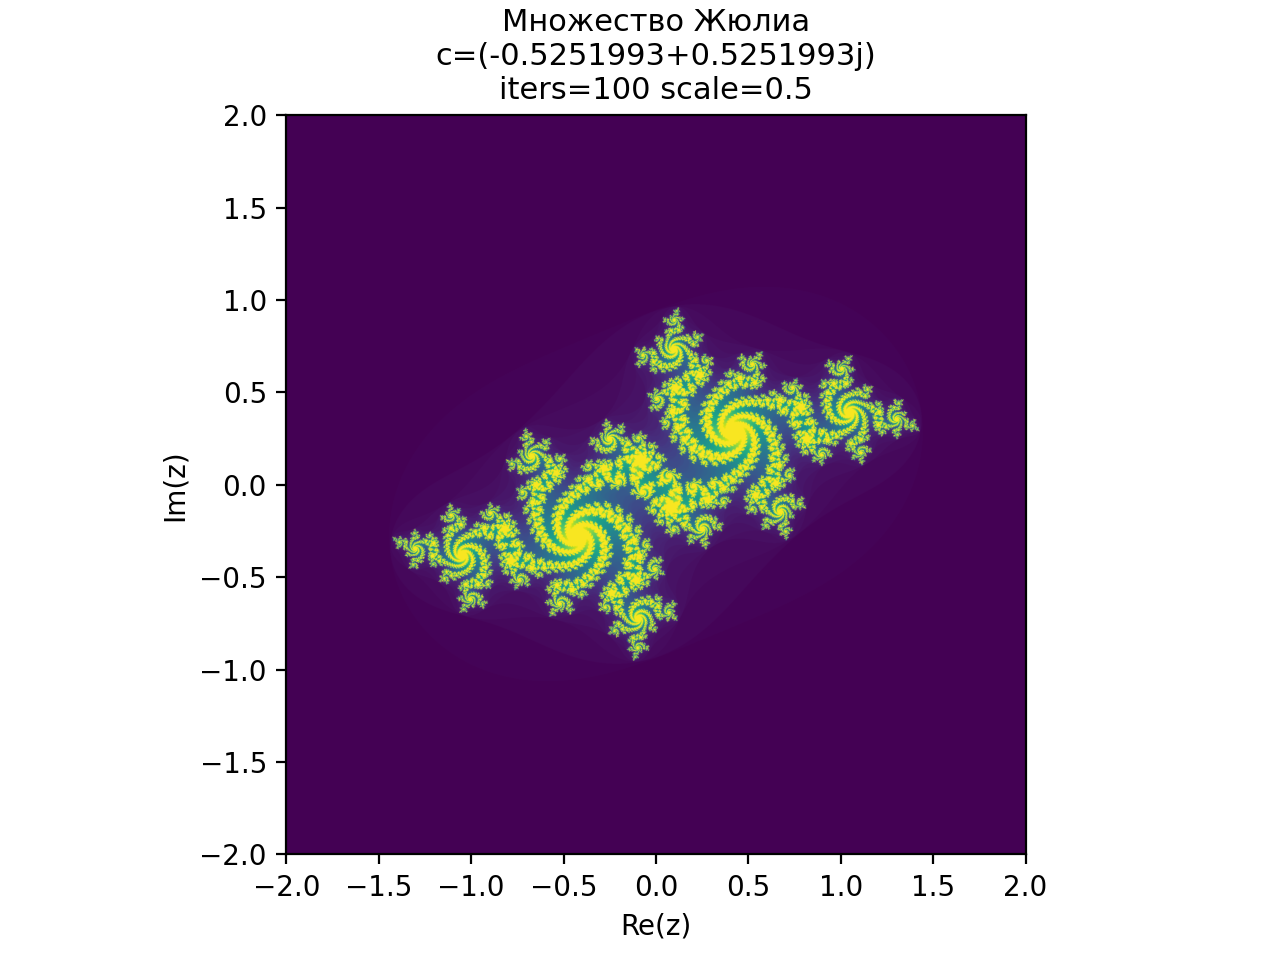
\includegraphics[width=0.9\textwidth]{julia_classic.png}
    
    \vspace{0.5cm}
    
    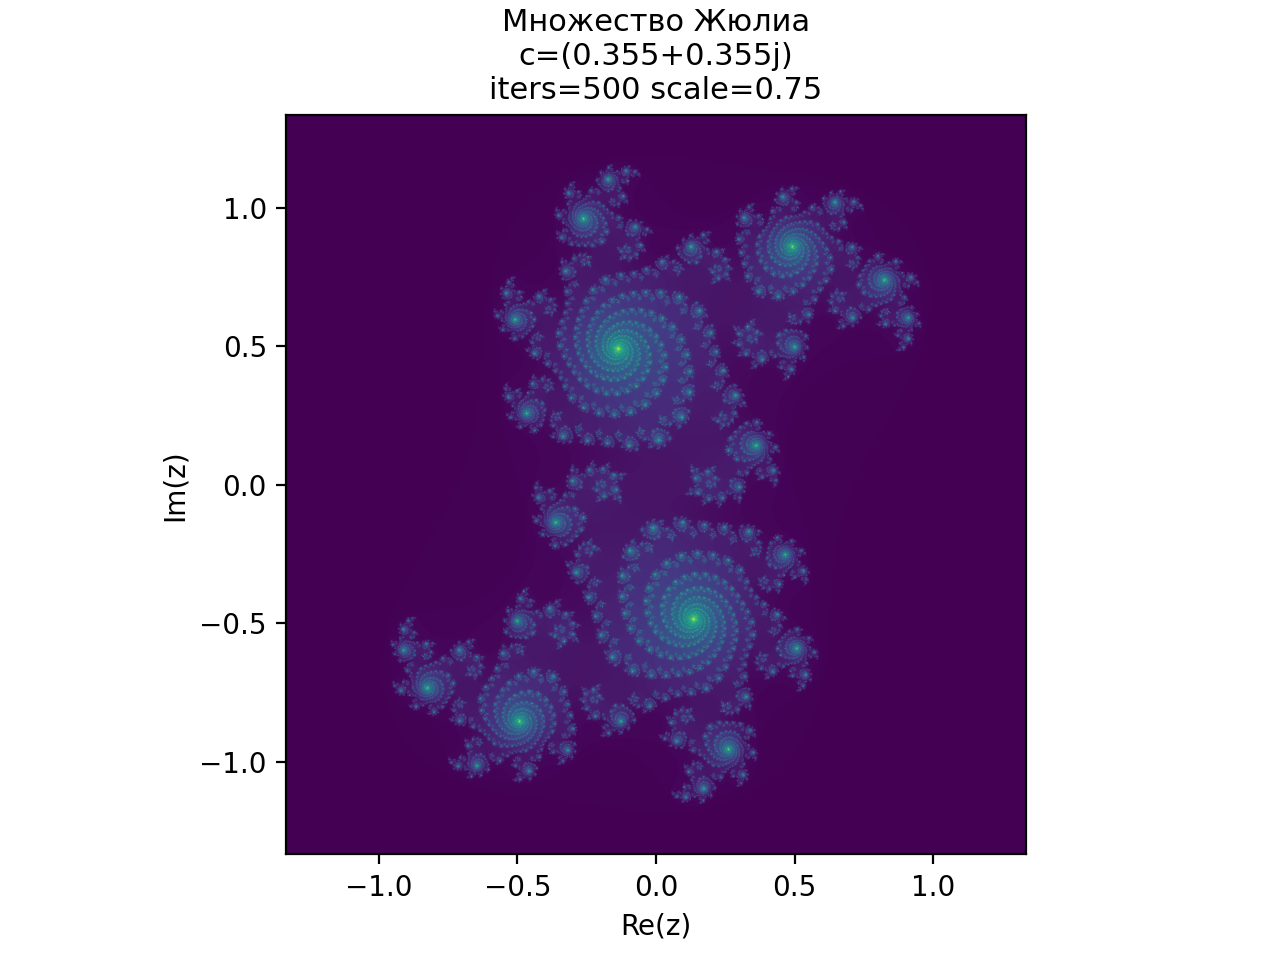
\includegraphics[width=0.9\textwidth]{julia_spirals.png}
\end{figure}

\clearpage

\begin{figure}[h!]
    \centering
    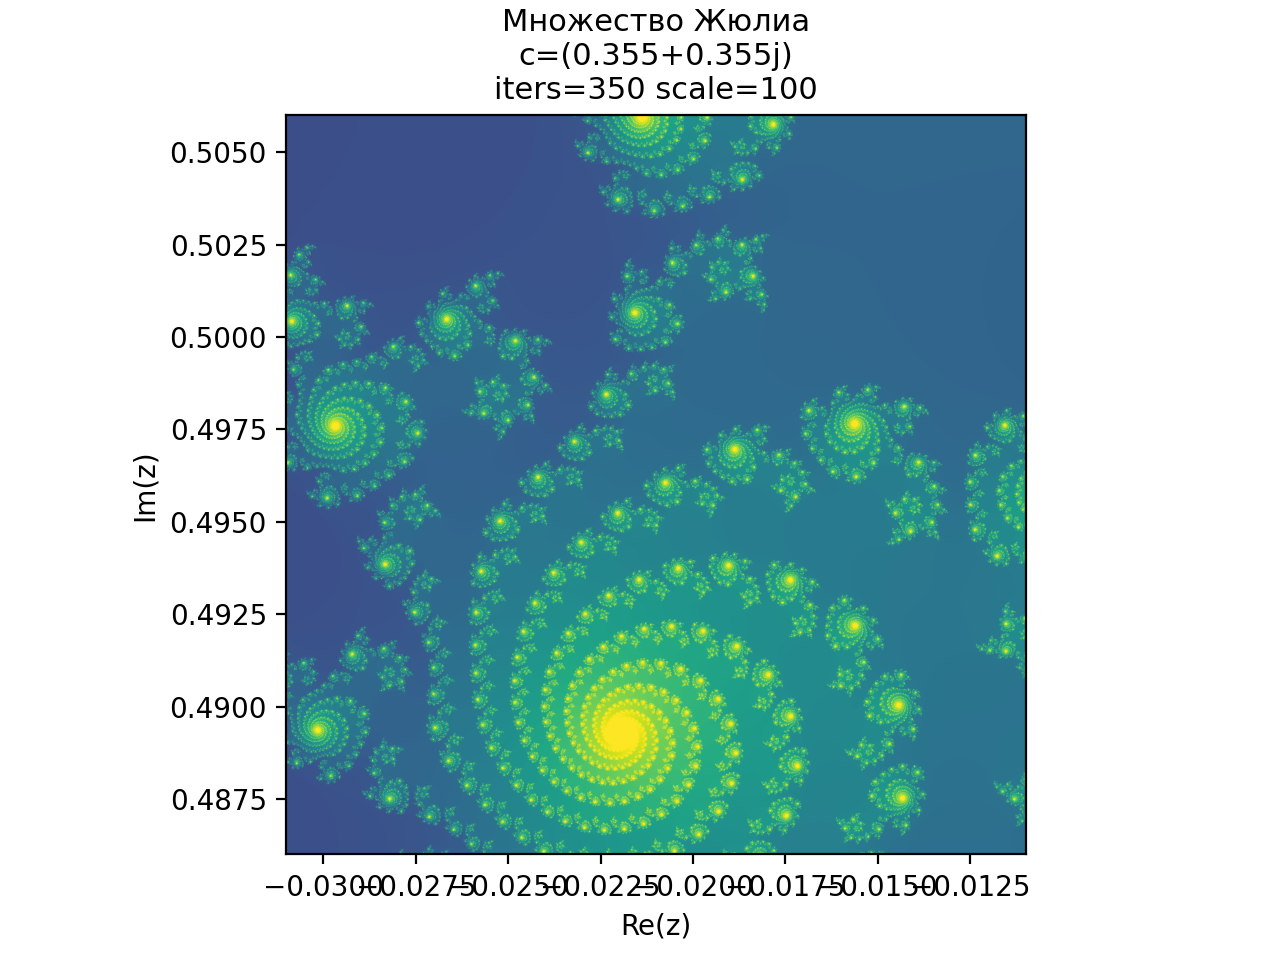
\includegraphics[width=1\textwidth]{julia_spirals_zoomed.png}
    
    \vspace{0.5cm}
    
    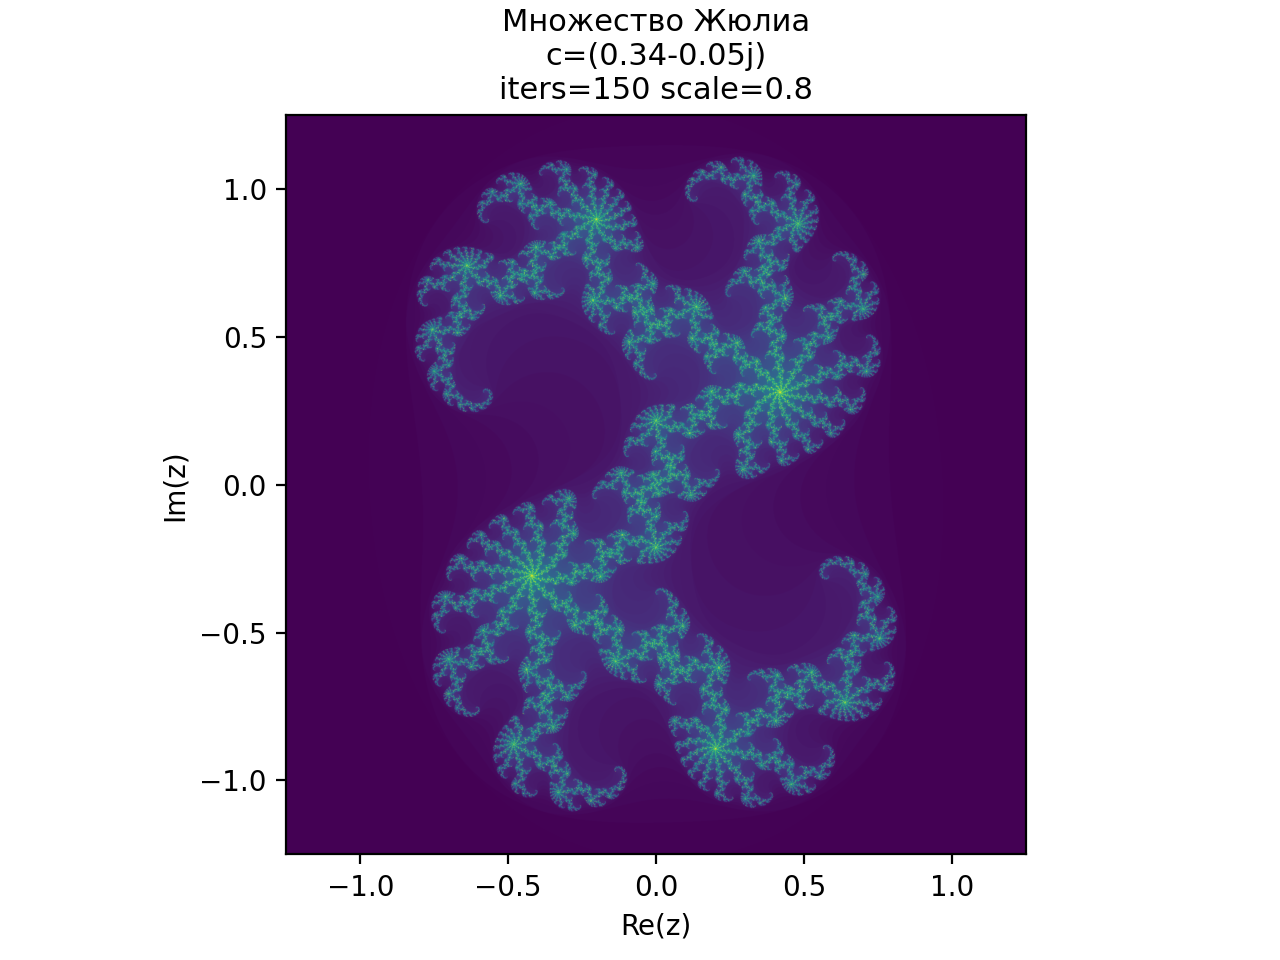
\includegraphics[width=1\textwidth]{julia_squid.png}
\end{figure}

\clearpage

\hypertarget{sec:8}{}
\section{\textbf{Фрактал «Горящий корабль»}}
В качестве неразобранного фрактала был выбран «Горящий корабль». Он был открыт Майклом Михеличем в 1992 году и является вариантом множества Мандельброта. Его структура отличается большей хаотичностью из-за небольшого изменения в итерационной формуле.

\subsection*{\textbf{Множество «Горящий корабль»}}
Рассмотрим последовательность комплексных чисел, заданную следующим образом:
$$ z_{n+1} = (|\text{Re}(z_n)| + i|\text{Im}(z_n)|)^2 + c, \quad \text{при } z_0 = 0 $$
Ключевое отличие от формулы для множества Мандельброта ($z_{n+1} = z_n^2 + c$) состоит в том, что перед возведением в квадрат на каждой итерации берутся абсолютные значения действительной и мнимой частей комплексного числа $z_n$.

\textbf{Определение.} Множество всех $c \in \mathbb{C}$, при которых заданная выше последовательность $z_n$ остается ограниченной, называется \textbf{множеством «Горящий корабль»}.

\subsection*{\textbf{Алгоритм построения}}
Алгоритм практически идентичен алгоритму построения множества Мандельброта:
\begin{enumerate}
    \item Берется ограниченная часть комплексной плоскости (например, от $-2 - 2i$ до $2 + 2i$), которая разбивается равномерной сеткой. Каждый узел сетки соответствует пикселю на изображении и представляет собой комплексное число $c$.
    \item Для каждой точки $c$ запускается итеративный процесс, начиная с $z_0 = 0$. Вводится ограничение на максимальное число итераций $M$ и условие «убегания»: если модуль $|z_n|$ превосходит 2, итерации прекращаются.
    \item Если после $M$ итераций последовательность не «убежала», считается, что точка $c$ принадлежит множеству, и соответствующий пиксель закрашивается в черный цвет.
    \item Для получения цветного изображения пиксели, не принадлежащие множеству, окрашиваются в цвет, зависящий от номера итерации, на которой произошло «убегание».
\end{enumerate}

\clearpage

\begin{lstlisting}[caption={Функция для построения множества "Горящий корабль"}, label={lst:burning_ship}]
def burning_ship_matrix(fractal_params, iterations, borders, density):
    z0 = fractal_params.get("z0")
    r = fractal_params.get("r")
    
    plane_start, plane_end = borders
    
    # Вектор действительных частей
    re_vec = np.linspace(plane_start.real, plane_end.real, density,
                         dtype=np.float64)
    
    # Вектор мнимых частей
    im_vec = np.linspace(plane_start.imag, plane_end.imag, density,
                         dtype=np.float64) * 1j
                         
    # Плоскость точек C
    plane = np.add.outer(im_vec, re_vec)
    
    # Результирующая матрица
    output = np.zeros(plane.shape, dtype='uint16')
    
    # Промежуточная матрица, заполненная z0
    z = np.full(plane.shape, z0, np.complex128)
    
    for i in range(iterations):
        # Маска точек, которые не "убежали"
        mask = np.less(np.abs(z), r)
        
        output[mask] = i
        
        # z_{n+1} = (|Re(z)| + i|Im(z)|)^2 + c
        z[mask] = (np.abs(z[mask].real) + 1j * np.abs(z[mask].imag))**2 + plane[mask]
        
    return output
\end{lstlisting}
Полный код вы можете увидеть на \href{https://github.com/Axe-On-You/tfkp-lab1}{Github}.

\clearpage

\begin{figure}[h!]
    \centering
    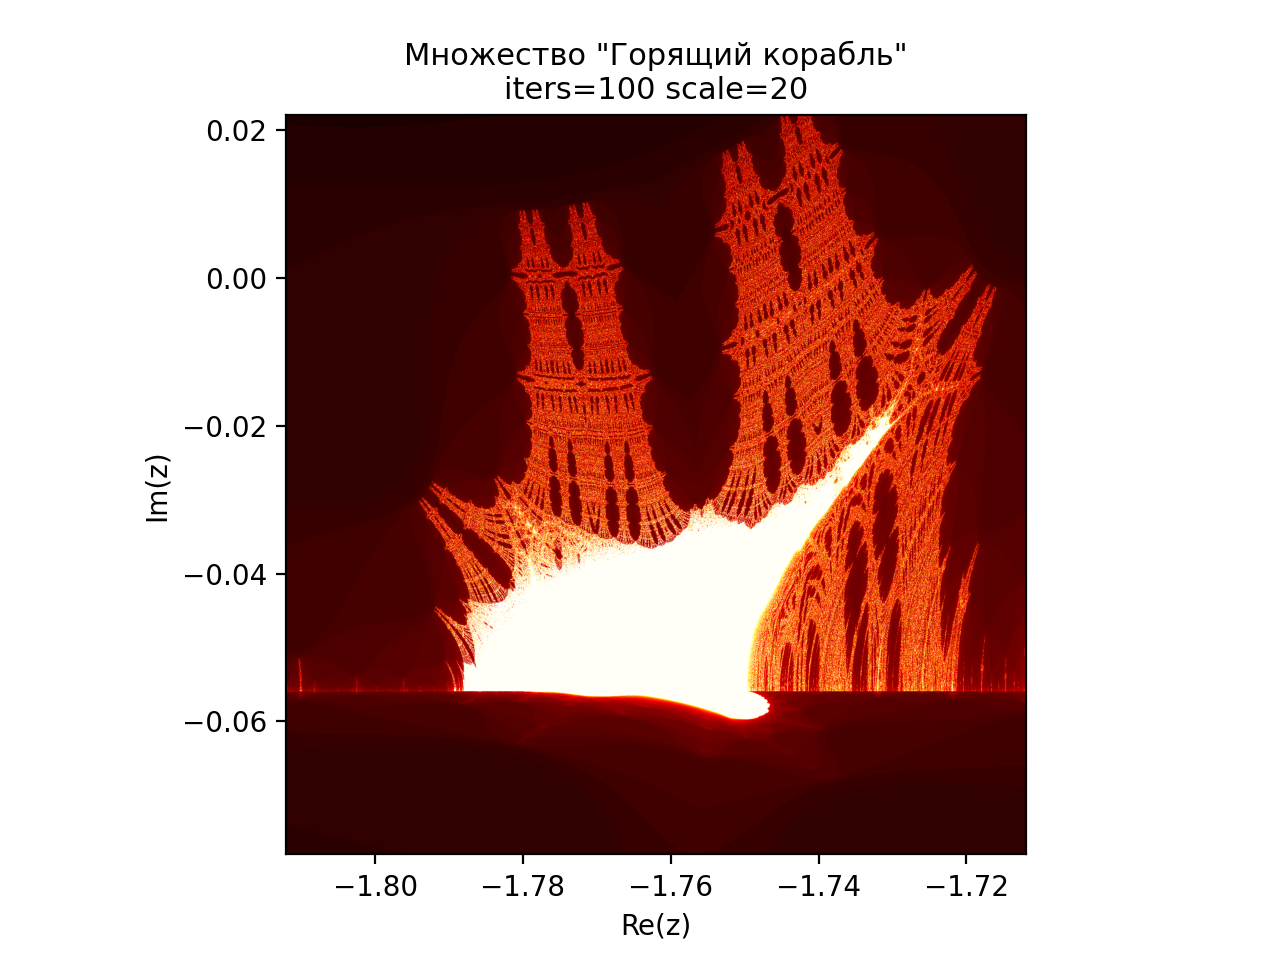
\includegraphics[width=0.9\textwidth]{ship_m_ship.png}
    
    \vspace{0.5cm}
    
    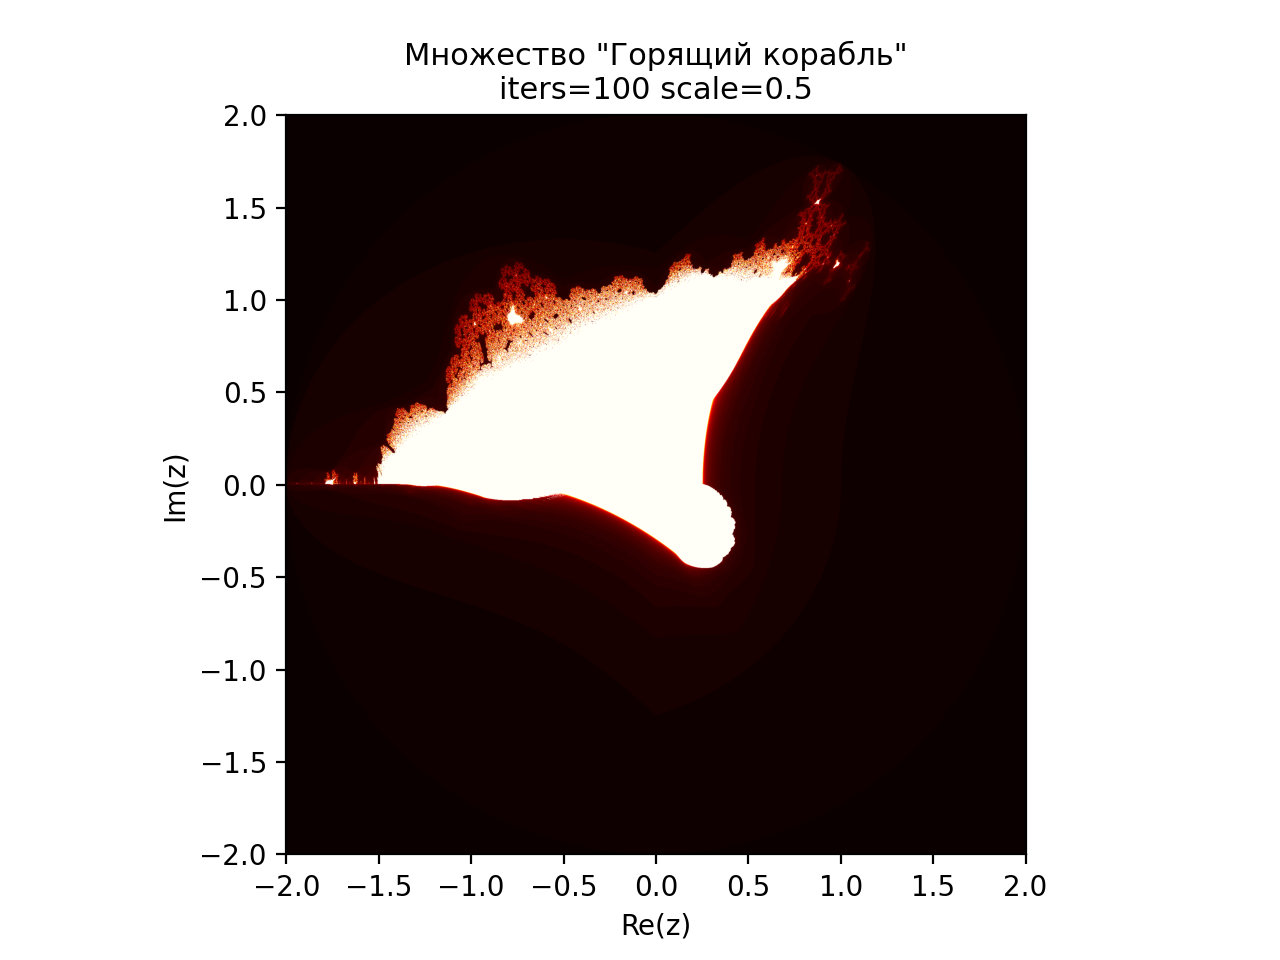
\includegraphics[width=0.9\textwidth]{ship_m_large.png}
\end{figure}

\clearpage

\begin{figure}[h!]
    \centering
    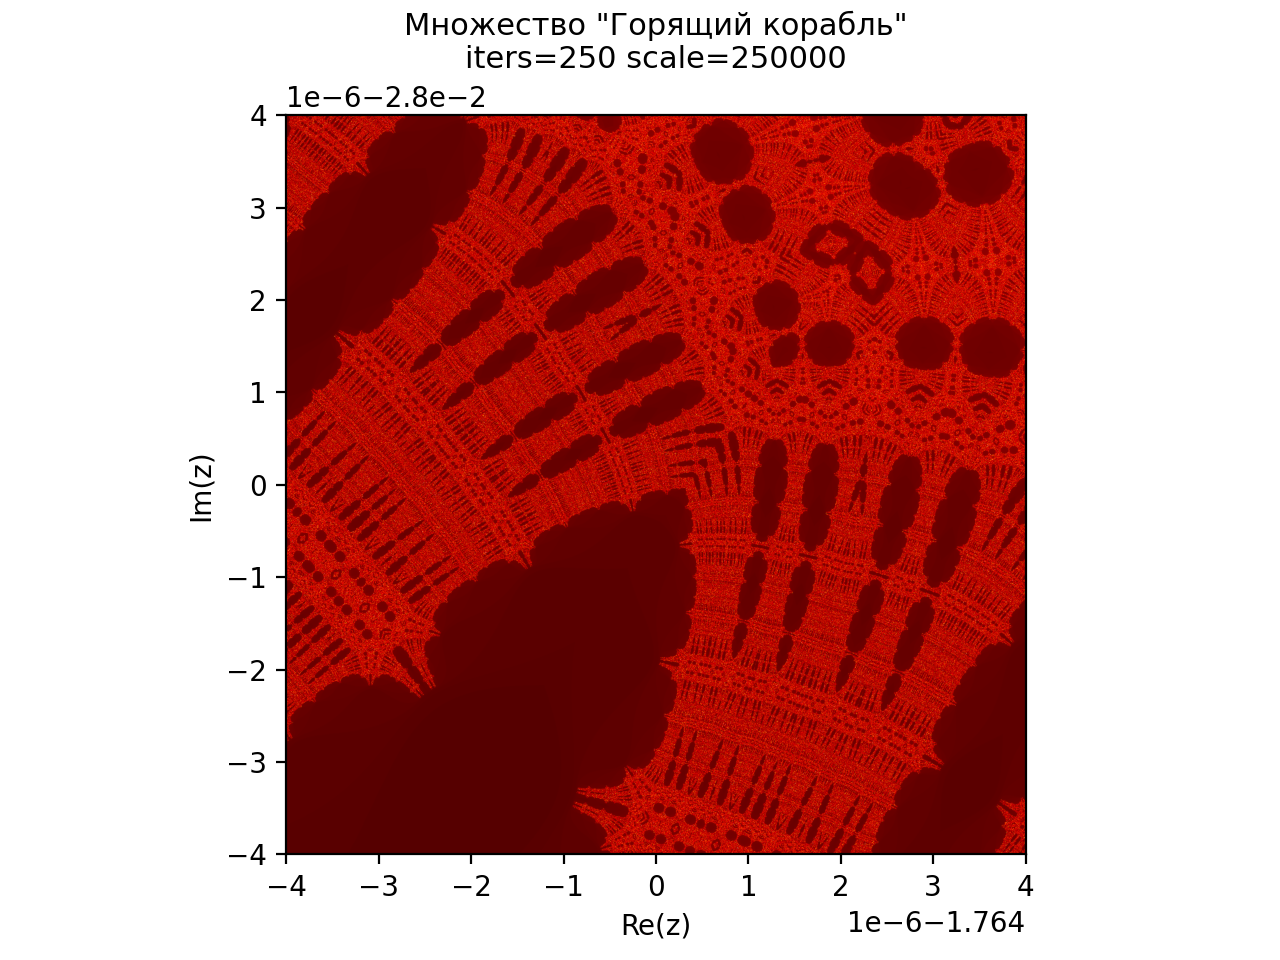
\includegraphics[width=1\textwidth]{ship_m_zoomed.png} 
\end{figure}

\end{document}